\subsection{Pipeline Visualization}
\label{sec:pipeline_visualization}

Visualizing pipeline execution is crucial for understanding task dependencies, debugging, optimizing workflows, and ensuring correct data flow within the LSST Science Pipelines.
To support this, \texttt{pipetask build} provides several options for visualizing the pipeline graph--a simplified directed acyclic graph that shows how tasks relate to dataset types, without including data IDs.

A text-based view can be generated using \texttt{pipetask build --show pipeline-graph}, which outputs an ASCII-style diagram.
This format is especially useful for quick inspection or when working in a terminal-only environment.
For graphical visualization, the \texttt{--pipeline-dot} and \texttt{--pipeline-mermaid} options export the pipeline graph in Graphviz DOT\footnote{\url{https://www.graphviz.org}} and Mermaid\footnote{\url{https://mermaid.js.org}} formats, respectively.
The Mermaid format is particularly well-suited for sharing in accessible, web-based contexts.

Unlike DOT files, which typically require rendering with external tools like Graphviz's \texttt{dot}, Mermaid definitions can be directly rendered in Markdown-based platforms such as GitHub, GitLab, some Jupyter environments, and even Slack with the appropriate plugin.
This makes Mermaid an effective format for generating interactive, easily shareable pipeline graphs that can be directly embedded in documentation, notebooks, or code review tools.

Figure~\ref{fig:pipe_viz} shows a visualization of a subset of two tasks from the \texttt{LSSTComCam/DRP-v2.yaml} pipeline using the Mermaid format.
The diagram shows the relationships between tasks and their input and output datasets as well as the sequence in which the tasks are expected to run.
Such visualizations can help uncover misconfigurations, missing inputs, or unexpected data dependencies that might otherwise result in issues such as empty QuantumGraphs or failed pipeline execution.

\begin{figure*}
    \centering
    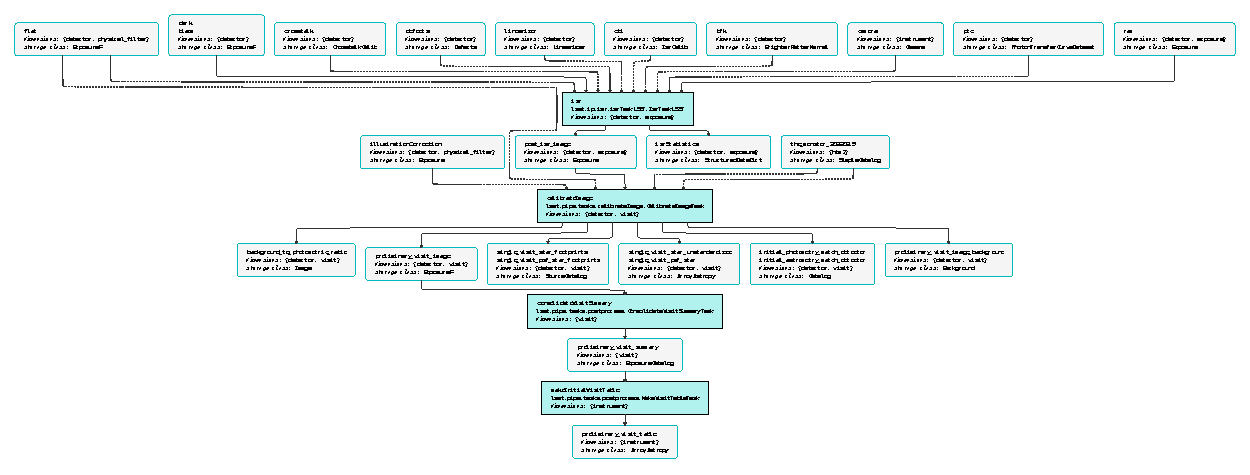
\includegraphics[width=\textwidth]{figures/pipe_viz_comcam_subset.pdf}
    \caption{
        Example pipeline visualization of four selected tasks from the \texttt{LSSTComCam/DRP-v2.yaml} pipeline in the Mermaid format.
        The diagram illustrates the flow of datasets between tasks, with dashed lines indicating prerequisite inputs.
        This visualization helps validate task dependencies and the expected sequence of execution.
    }
    \label{fig:pipe_viz}
\end{figure*}
